\documentclass[useAMS,usenatbib]{mn2e}

%%%%% AUTHORS - PLACE YOUR OWN MACROS HERE %%%%%
\newcommand{\conj}[1]{\overline{#1}}
\newcounter{NameOfTheNewCounter}
\setcounter{NameOfTheNewCounter}{1}
\newtheorem{theorem}{Theorem}[NameOfTheNewCounter]
\newtheorem{lemma}[theorem]{Lemma}
\newtheorem{proposition}[theorem]{Proposition}
\newtheorem{corollary}[theorem]{Corollary}
\newtheorem{definition}[theorem]{Definition}
\newtheorem{conjecture}[theorem]{Conjecture}
\usepackage{graphicx}
\usepackage{amsfonts}
\newcommand{\Gcal}{\bmath{\mathcal{G}}}
\newcommand{\Rcal}{\bmath{\mathcal{R}}}
\newcommand{\Mcal}{\bmath{\mathcal{M}}}
\newcommand{\Fcal}{\bmath{\mathcal{F}}}

\newcommand{\COMPLEX}{\mathbb{C}}
\newcommand{\REAL}{\mathbb{R}}
\newcommand{\II}{\mathbb{I}}

\newcommand{\zz}{\bmath{z}}

\newcommand{\mat}[1]{{\bmath{#1}}}

\newcommand{\JJ}{\mat{J}} % \bmath{\mathcal{J}}}
\newcommand{\DD}{\mat{D}}
\newcommand{\MM}{\mat{M}}
\newcommand{\RR}{\mat{R}}
\newcommand{\LL}{\mat{L}}
\newcommand{\RHO}{\mat{\Rho}}
\newcommand{\GG}{\mat{G}}
\newcommand{\JHJ}{\JJ^H\JJ} % \bmath{\mathcal{J}}}

\newcommand{\aaps}{A\&AS}
\newcommand{\aap}{A\&A}
\newcommand{\mnras}{MNRAS}
\newcommand{\nat}{Nature}
\newcommand{\physrep}{Phys. Rep.}

%%%%%%%%%%%%%%%%%%%%%%%%%%%%%%%%%%%%%%%%%%%%%%%%

\title[Complex optimization for radio interferometeric calibration]{Complex optimization for radio interferometeric calibration}
\author[N. Bourbaki]{N. Bourbaki$^1$\thanks{E-mail: nbourbaki@pantheon.fr}\\ 
$^1$Institute For The Advancement Of Complex Chicken Recipes}
\begin{document}

\date{in original form 2014 February 2}

\pagerange{\pageref{firstpage}--\pageref{lastpage}} \pubyear{2014}

\maketitle

\label{firstpage}

\begin{abstract}
\end{abstract}

\begin{keywords}
Instrumentation: interferometers, Methods: analytical, Methods: numerical, Techniques: interferometric
\end{keywords}

\section{Introduction}

Chicken chicken chicken. Chicken chicken? Chicken\footnote{Chicken chicken!} chicken, chicken (Chicken \& Chicken 2014).

\section{Complex optimization \& Wirtinger calculus}

The traditional approach to optimizing a function of $n$ complex variables $f(\zz),$ $\zz\in\COMPLEX^n$ is
to treat the real and imaginary parts $\zz=\bmath{x}+i\bmath{y}$ independently, turning $f$ into a function
of $2n$ real variables $f(\bmath{x},\bmath{y})$, and the problem into an optimization over $\REAL^{2n}$.

\citet{ComplexOpt} have developed an alternative approach to the problem based on Wirtinger calculus. The central idea
of Wirtinger calculus is to treat $\zz$ and $\bar{\zz}$ as independent variables, and optimize $f(\zz,\bar{\zz})$
using the Wirtinger derivatives 

\[
\frac{\partial}{\partial z} = \frac{1}{2}\left ( \frac{\partial}{\partial x} - i\frac{\partial}{\partial y} \right),~~
\frac{\partial}{\partial \bar{z}} = \frac{1}{2}\left ( \frac{\partial}{\partial x} + i\frac{\partial}{\partial y} \right),
\]
where $z=x+iy$. It is easy to see that  
\[
\frac{\partial \bar z}{\partial z} = 
\frac{\partial z}{\partial \bar z} = 0,
\]
i.e. that $\bar z$ ($z$) is treated as constant when taking the derivative with respect to $z$ ($\bar z$). From this 
it is straightforward to define the \emph{complex gradient} operator 

\[
\frac{\partial}{\partial^C \zz} = \left [ \frac{\partial}{\partial \zz} \frac{\partial}{\partial \bar{\zz}} \right ] = \left [ \frac{\partial}{\partial z_1} \cdots \frac{\partial}{\partial z_n}
\frac{\partial}{\partial \bar{z}_1} \cdots \frac{\partial}{\partial \bar{z}_n} \right ],
\]

from which definitions of the complex Jacobian and complex Hessians naturally follow. The authors then show 
that various optimization techniques developed for real functions can be reformulated using 
complex Jacobians and Hessians, and applied to the complex optimization problem. Of particular interest to 
us, they generalize the Levenberg-Marquardt method for solving the the non-linear least squares (LS) problem

\begin{equation}
\label{eq:LSmin}
\min_{\bmath{z}} ||\bmath{r}(\bmath{z},\bmath{\bar z})||_F,
\end{equation}

where $\bmath{r}$ has values in $\COMPLEX^m$, and $||\cdot||_F$ is the Frobenius norm. This is done as follows.
Let $\zz_k$ be the parameter vector at step $k$. Then, define

\newcommand{\Matrix}[2]{\left [ \begin{array}{@{}#1@{}}#2\end{array} \right ]}
\newcommand{\Stack}[1]{\begin{array}{@{}c@{}}#1\end{array}}

\begin{equation}
\label{eq:Jk}
\JJ_k=\frac{\partial \bmath{r}}{\partial \zz} (\zz_k,\bar{\zz}_k), ~\JJ_{\bar{k}}=\frac{\partial \bmath{r}}{\partial \bar{\zz}}(\zz_k,\bar{\zz}_k),~\bmath{r}_k=\Matrix{c}{\bmath{r}(\zz_k,\bar{\zz}_k)\\\bar{\bmath{r}}(\zz_k,\bar{\zz}_k)}
\end{equation}

We'll call the $m\times n$ matrices $\JJ_k$ and $\JJ_{\bar{k}}$ the \emph{partial} and \emph{partial conjugate Jacobian}, respectively, 
and the $2m$-vector $\bmath{r}_k$ the \emph{augmented residual vector}. The \emph{complex Jacobian} 
of the cost function $||\bmath{r}(\bmath{z},\bmath{\bar z})||^2$ can then be written (in block matrix form) as

\begin{equation}
\label{eq:JJ}
\JJ = \Matrix{cc}{J_k & J_{\bar{k}} \\ \bar{J}_{\bar{k}} & \bar{J}_k },
\end{equation}

Note that this is a $2m \times 2n$ matrix. The LM parameter update step is then defined as

\begin{equation}
\label{eq:LM}
\Matrix{c}{\delta \zz \\ \delta \bar{\zz}} = -(\JJ^H \JJ + \lambda\II)^{-1}\JJ^H \bmath{r}_k,
\end{equation}

where $\II$ is the identity matrix, and $\lambda$ is the LM damping parameter. When $\lambda=0$ this becomes 
equivalent to the Gauss-Newton (GN) method; with $\lambda\to\infty$ this corresponds to steepest descent with ever smaller steps.

An alternative version of LM is formulated as

\begin{equation}
\label{eq:LM1}
\Matrix{c}{\delta \zz \\ \delta \bar{\zz}} = -(\JJ^H \JJ + \lambda \DD)^{-1}\JJ^H \bmath{r}_k,
\end{equation}

where $\DD$ is simply the diagonalized version of $\JJ^H\JJ$.

\citet{ComplexOpt} show that Eq.~\ref{eq:LM} yields exactly the same system of LS equations as would have 
been produced had we treated $\bmath{r}$ as a function of real and imaginary parts $\bmath{r}(\bmath{x},\bmath{y})$, 
and taken ordinary derivatives in $\REAL^{2n}$. However, the complex Jacobian may be easier and more elegant 
to derive analytically, as we'll see below in the case of radio interferometric calibration.

\section{Unpolarized direction independent calibration}

\newcommand{\Na}{N_\mathrm{ant}}
\newcommand{\Nbl}{N_\mathrm{bl}}
\newcommand{\Nd}{N_\mathrm{dir}}

Let us first consider the simplest case, that of unpolarized direction-independent (DI) calibration. Consider an interferometer
array of $\Na$ antennas measuring $\Nbl=\Na(\Na-1)/2$ pairwise visibilities. Each antenna pair $pq$ ($1\leq p<q\leq \Na$) 
measures the visibility

\begin{equation}
\label{eq:RIME:unpol}
g_p m_{pq} \bar{g}_q + n_{pq},
\end{equation}

where $m_{pq}$ is the (assumed known) sky coherency, $g_p$ is the (unknown) complex gain parameter 
associated with antenna $p$, and $n_{pq}$ is a complex noise term that is Gaussian with a mean of 0 in the real and 
imaginary parts. The calibration problem then consists of estimating the complex antenna gains $\bmath{g}$ by
minimizing residuals in the LS sense:

\begin{equation}
\label{eq:cal:DI}
\min_{\bmath{g}}\sum_{pq}|r_{pq}|^2,~~~r_{pq}=d_{pq}-g_p m_{pq} \bar{g}_q, 
\end{equation}

where $d_{pq}$ are the observed visibilities. Treating this as a complex optimization problem as per the above, 
let us write out the complex Jacobian. 
We have a vector of $\Na$ complex unknowns $\bmath{g}$ and $\Nbl$ measurements $d_{pq}$, the full complex
Jacobian will then have a shape of $2\Nbl\times2\Na$. It is conventional
to think of visibilities laid out in a visibility matrix; the normal approach at this stage is to vectorize $d_{pq}$ 
by fixing a numbering convention so as to enumerate all the possible antenna pairs $pq$ ($p<q$) using numbers from 1 to $\Nbl$.
Instead, let us keep using $pq$ as a single ``compound index'', with the implicit understanding that $pq$ in 
subscript corresponds to a single index from 1 to $\Nbl$ using \emph{some} fixed enumeration convention. 
Where necessary, we'll write $pq$ in square brackets (e.g. $a_{[pq],i}$) to emphasize this.

Now consider the patrial Jacobian $\JJ_k$ matrix in Eq.~\ref{eq:Jk}. This is of shape $\Nbl\times\Na$. We can write the
partial Jacobian in terms of its value at row $[pq]$ and column $j$ as 

\[
[ \JJ_k ]_{[pq],j} = \left \{  
  \begin{array}{ll} 
  -m_{pq}\bar{g}_q,& j=p, \\
  0, & \mathrm{otherwise.}
  \end{array}
\right .
\]

In other words, within each column $j$, $J_k$ is only non-zero at rows corresponding to baselines $[jq]$. We can express 
this more compactly using the Kronecker delta:


\[
J_k = - \overbrace{ \Matrix{c}{ m_{pq}\bar{g}_q\delta^{j}_p } } ^{j=1\dots \Na} \big \}{\scriptstyle [pq]=1\dots \Nbl~(p<q)}
\]

Likewise, the conjugate partial Jacobian $\JJ_{\bar{k}}$ may be written as

\[
J_{\bar{k}} = - \overbrace{ \Matrix{c}{ g_p m_{pq} \delta^{j}_q } } ^{j=1\dots \Na} \big \}{\scriptstyle [pq]=1\dots \Nbl~(p<q)}
\]

To give a specific example, for 3 antennas, using the numbering convention for $pq$ of
12, 13, 32, we have:

\[
\JJ_k = - \Matrix{ccc}{m_{12}\bar{g}_2 & 0 & 0 \\ m_{13}\bar{g}_3 & 0 & 0 \\ 0 & m_{23}\bar{g}_3 & 0 },
\JJ_{\bar{k}} = - \Matrix{ccc}{0 & g_1 m_{12} & 0 \\ 0 & 0 & g_1 m_{13} \\ 0 & 0 & g_2 m_{23} }
\]


The full complex Jacobian (Eq.~\ref{eq:JJ}) then becomes, in block matrix notation,

\begin{equation}
\label{eq:JJ:di:basic}
\begin{array}{r@{~}cc@{~}cc}
                & \overbrace{~~~~~~~~}^{j=1\dots \Na} & \overbrace{~~~~~~~~}^{j=1\dots \Na} \\
\JJ = - \bigg [ &
  \Stack{ m_{pq}\bar{g}_q\delta^{j}_p \\ \bar{m}_{pq} \bar{g}_p \delta^{j}_q } &
  \Stack{ g_p m_{pq} \delta^{j}_q \\ g_q \bar{m}_{pq} \delta^{j}_p }  
& \bigg ] &
\Stack{ \} {\scriptstyle [pq]=1\dots \Nbl}~(p<q) \\ \} {\scriptstyle [pq]=1\dots \Nbl}~(p<q) }

\end{array}
\end{equation}

where the $[pq]~(p<q)$ and $j$ subscripts within each block span the full range of $1\dots \Nbl$ and $1\dots \Na$. Now, 
since $d_{pq} = \bar{d}_{qp}$ and $m_{pq} = \bar{m}_{qp}$, we may notice
that the bottom half of the augumented residuals vector $\bmath{r}$ corresponds to the conjugate baselines 
$qp$ ($q>p$):


\[
\bmath{r} = \Matrix{c}{ r_{pq} \\ \bar{r}_{pq} } = \Matrix{c}{d_{pq}-g_p m_{pq}\bar{g}_q\\ \bar{d}_{pq}-\bar{g}_p \bar{m}_{pq}g_q} = 
\Matrix{c}{ r_{pq} \\ r_{qp} }~~ 
\Stack{ \} \scriptstyle [pq]=1\dots \Nbl~(p<q) \\ \} \scriptstyle [pq]=1\dots \Nbl~(p<q) }
\]

as does the bottom half of $\JJ$ in Eq.~\ref{eq:JJ:di:basic}. Note that we are free to reorder the rows of $\JJ$ and $\bmath{r}$ 
and intermix the normal and conjugate baselines, as this will not affect the LS equations derived at Eq.~\ref{eq:LM}.
This proves most convenient: instead of splitting $\JJ$ and $\bmath{r}$ into 
two vertical blocks with the compound index $[pq]~(p<q)$ running through $\Nbl$ rows within each block, we can treat 
the two blocks as one, with a single compound index $[pq]~(p\ne q)$ running through $2\Nbl$ rows:

\begin{equation}
\label{eq:JJ:di}
\begin{array}{r@{~}cc@{~}cc}
                & \overbrace{~~~~~~~~}^{j=1\dots \Na} & \overbrace{~~~~~~~~}^{j=1\dots \Na} \\
\JJ = - \big [ & m_{pq}\bar{g}_q\delta^{j}_p & g_p m_{pq} \delta^{j}_q & \big ],~
\bmath{r} = \big [ r_{pq} \big ] ~~{\} \scriptstyle [pq]=1\dots 2\Nbl}
\end{array}
\end{equation}

where for $q>p$, $r_{pq}=\bar{r}_{qp}$ and $m_{pq}=\bar{m}_{qp}$. For clarity, we may adopt the 
following order for enumerating the row index $[pq]$: $12,13,\dots,1n,$ $21,22,\dots,2n,$ $31,32,\dots,3n,$ $\dots,n1,\dots,n\,n-1$. 
For example, the complex Jacobian $\JJ$ for the 3-antenna case would then look like:

\[
-\Matrix{cccccc}{
  m_{12}\bar{g}_2 & 0               & 0 &  0          & g_1 m_{12} & 0           \\
  m_{13}\bar{g}_3 & 0               & 0 &  0          & 0          & g_1 m_{13}  \\
  0               & m_{21}\bar{g}_1 & 0 &  g_2 m_{21} & 0          & 0  \\
  0               & m_{23}\bar{g}_3 & 0 &  0          & 0          & g_2 m_{23} \\
  0               & 0               & m_{31}\bar{g}_1 & g_1 m_{31} & 0          & 0  \\
  0               & 0               & m_{32}\bar{g}_2 & 0 & g_3 m_{32} & 0 \\
}
\]


For brevity, let us define the shorthand $y_{pq} = m_{pq} \bar{g}_q$. 
We can now write out the structure of $\JJ^H\JJ$. This is Hermitian, consisting of four $\Na\times\Na$ blocks:

\[
\JJ^H\JJ = \Matrix{cc}{\mat{A}&\mat{B}\\\mat{C}&\mat{D}} = \Matrix{cc}{\mat{A}&\mat{B}\\\mat{B}^H&\mat{A}}
\]

since the value at row $i$, column $j$ of each block is
\begin{eqnarray}
A_{ij} = \sum_{pq} \bar{y}_{pq} y_{pq} \delta^{i}_p \delta^{j}_p &=& 
  \left \{ \begin{array}{cc}
        \sum\limits_{q\ne i} |y_{pq}^2|, & \scriptstyle i=j \\
        0,  & \scriptstyle  i\ne j
  \end{array} \right .\nonumber\\ 
B_{ij} = \sum_{pq} \bar{y}_{pq} \bar{y}_{qp} \delta^{i}_p \delta^{j}_q &=& 
  \left \{ \begin{array}{cc}
      \bar{y}_{pq} \bar{y}_{qp}, & \scriptstyle i\ne j\\
      0, & \scriptstyle i=j
  \end{array} \right .\nonumber\\ 
C_{ij} = \sum_{pq} y_{qp} y_{pq} \delta^{i}_q \delta^{j}_p &=& 
  \bar{B}_{ij} \nonumber\\
D_{ij} = \sum_{pq} y_{pq} \bar{y}_{pq} \delta^{i}_q \delta^{j}_q &=& A_{ij} 
\label{eq:JHJ:DI:ABCD}
\end{eqnarray}

We then write $\JJ^H\JJ$ in terms of the four $\Na\times\Na$ blocks as:

\begin{equation}
\label{eq:JHJ:DI}
\JJ^H \JJ = \Matrix{c@{~\bigg |~}c}{
\mathrm{diag} \sum\limits_{q\ne i} |y_{iq}^2| & 
  \left \{ 
  \begin{array}{@{}cc@{}}
   \bar{y}_{ij} \bar{y}_{ji}, &{\scriptstyle i\ne j} \\
   0, &{\scriptstyle i=j}
  \end{array} \right .\\
  \left \{ 
  \begin{array}{@{}cc@{}}
   y_{ij}y_{ji},&{\scriptstyle i\ne j} \\
   0, &{\scriptstyle i=j}
  \end{array} \right . 
  & \mathrm{diag} \sum\limits_{q\ne i} |y^2_{iq}| 
}
% \Stack{ 
% \bigg \} \scriptstyle i=1\dots \Na \\ 
% \bigg \} \scriptstyle i=1\dots \Na 
%}
\end{equation}

For example, in the 3-antenna case, we have the following expression for
$\JJ^H \JJ$:

\newcommand{\yysq}[2]{{y^2_{#1}+y^2_{#2}}}
\newcommand{\bb}[2]{{\bar{y}_{#1#2}\bar{y}_{#2#1}}}
\newcommand{\bbb}[2]{y_{#1#2}y_{#2#1}}
\begin{equation}
\label{eq:JHJ:3ant}
{\scriptstyle
\Matrix{c@{}c@{}c@{}c@{}c@{}c}{
\yysq{12}{13} & 0             & 0             & 0             & \bb{1}{2}       & \bb{1}{3} \\
0             & \yysq{12}{23} & 0             & \bb{1}{2}       & 0             & \bb{2}{3} \\
0             & 0             & \yysq{13}{23} & \bb{1}{3}       & \bb{2}{3}       & 0       \\
0             & \bbb{1}{2}      & \bbb{1}{3}      & \yysq{12}{13} & 0             & 0       \\ 
\bbb{1}{2}      & 0             & \bbb{2}{3}      & 0             & \yysq{12}{23} & 0 \\
\bbb{1}{3}      & \bbb{2}{3}      & 0             & 0             & 0             &  \yysq{13}{23}  
}
}
\end{equation}

The other component of the LM equations (Eq.~\ref{eq:LM}) is the $\JJ^H\bmath{r}$ term. This will be a column
vector of length $2\Na$. We can write this as a stack of two $\Na$-vectors:


\begin{equation}
\label{eq:JHR:DI}
\JJ^H\bmath{r} = -\Matrix{c}{ 
\sum\limits_{pq} \bar{y}_{pq} r_{pq} \delta^{i}_p  \\
\sum\limits_{pq} y_{qp} r_{pq} \delta^{i}_q 
} = -\Matrix{c}{
\sum\limits_{q\ne i} \bar{y}_{iq} r_{iq}   \\
\sum\limits_{q\ne i} y_{iq} \bar{r}_{iq}  
}
\Stack{
\big \} \scriptstyle i=1\dots \Na \\ 
\big \} \scriptstyle i=1\dots \Na,
}
\end{equation}

with the second equality established by swapping $p$ and $q$ in the bottom sum, and making use of $y_{pq}=\bar{y}_{qp}$ and $r_{pq}=\bar{r}_{qp}$. Clearly, the bottom vector is the conjugate of the top:

\begin{equation}
\label{eq:JHR:DI1}
\JJ^H\bmath{r} = -\Matrix{c}{\bmath{c}\\\bar{\bmath{c}}},~~c_i = \sum\limits_{q\ne i} \bar{y}_{iq} r_{iq}.
\end{equation}

Equations~\ref{eq:JHJ:DI} and \ref{eq:JHR:DI1} give us the necessary ingredients for implementing complex
optimization of the RIME using LM, GN and/or steepest descent. 

\subsection{Diagonal approximation and Stefcal}
\label{sec:DI:stefcal}

A naive implementation of LS or GN above would hinge on inverting a $2\Na\times2\Na$ matrix, which is generally 
an $O(\Na^3)$ operation. However, the structure of $\JJ^H\JJ$ in Eq.~\ref{eq:JHJ:DI} suggests that it is diagonally 
dominant (especially for larger $\Na$), as the diagonal terms are added coherently. It is therefore not unreasonable 
to try approximating it with a diagonal matrix for purposes of inversion, thus making the problem separable per antenna,
and making matrix inversion itself negligible ($O(\Na)$ cost, as opposed to the $O(\Na^2)$ cost of computing the 
diagonal elements of the Jacobian in the first place). The cost of using an approximation for $\JHJ$ is a less accurate
update step, so we can expect to require more iterations before convergence is reached.

Applying this idea to Eq.~\ref{eq:LM} with $\lambda=0$ (i.e. implementing GN minimization), we end up with a 
simple per-antenna equation for computing the $\bmath{g}$ update step:

\begin{equation}
\label{eq:update:di:unpol}
\delta g_p = \left( \sum\limits_{q\ne p} |y^2_{pq}|  \right )^{-1} \sum\limits_{q\ne p} \bar{y}_{pq} r_{pq},
\end{equation}

Even more elegantly, the updated parameter estimate $\hat{\bmath{g}} = \bmath{g}+\delta \bmath{g}$ can be written as

\begin{equation}
\label{eq:stefcal}
\hat{g}_p = g_p + \frac{\sum\limits_{q\ne p} \bar{y}_{pq} (d_{pq} - g_p y_{pq})}{\sum\limits_{q\ne p} \bar{y}_{pq} y_{pq}} 
= \frac{\sum\limits_{q\ne p} \bar{y}_{pq} d_{pq} }{\sum\limits_{q\ne p} \bar{y}_{pq} y_{pq}},
\end{equation}

which eliminates the need to actually compute residuals. This is identical to the update step proposed by \citet{Stefcal} for the 
Stefcal algorithm, and by \citet{Mitchell-RTS} for MWA calibration. Note that these authors arrive at the equation from a different 
direction, by treating Eq.~\ref{eq:cal:DI} as a function of $\bmath{g}$ only, and ignoring the conjugate term. The 
resulting complex Jacobian (Eq.~\ref{eq:JJ:di:basic}) will then have null off-diagonal blocks, and $\JJ^H\JJ$ becomes 
diagonal.

Interestingly, if we use the diagonal $\JJ^H\JJ$ approximation with the modified LM method of Eq.~\ref{eq:LM1}, we instead 
arrive at

\[
\hat{g}_p = \frac{\lambda}{1+\lambda}g_p + \frac{1}{1+\lambda} \frac{\sum\limits_{q\ne p} \bar{y}_{pq} d_{pq}}{
\sum\limits_{q\ne p} \bar{y}_{pq} y_{pq}}
\]

which for $\lambda=1$ essentially becomes the basic average-update step of Stefcal.

Establishing the equivalence between Stefcal and complex optimization with a diagonally-approximated $\JJ^H\JJ$ is 
very useful for our purposes, since the convergence properties of Stefcal have been thoroughly explored 
by \citet{Stefcal}, and we can therefore hope to apply these lessons here. In particular, these authors have shown 
that a direct application of Eq.~\ref{eq:stefcal} leads to very slow convergence, whereas averaging every pair of 
updates leads to faster convergence. They also propose a number of variations of the algorithm, all of which are 
directly applicable to the above.

\subsection{Weighting}
\label{sec:DI:W}

Although \citet{ComplexOpt} do not mention this explicitly, it is straightforward to incorporate weights into the 
complex LS problem. Equation~\ref{eq:LSmin} is reformulated as

\begin{equation}
\label{eq:LSmin:w}
\min_{\bmath{z}} ||\mat{W} \bmath{r}(\bmath{z},\bmath{\bar z})||_F,
\end{equation}

where $\mat{W}$ is an $M\times M$ weights matrix (usually, the inverse of the data covariance matrix $\mat{C}$). This then propagates into the 
LM equations as

\begin{equation}
\label{eq:LM:W}
\Matrix{c}{\delta \zz \\ \delta \bar{\zz}} = -(\JJ^H \mat{W} \JJ + \lambda\II)^{-1}\JJ^H \mat{W} \bmath{r}_k,
\end{equation}

To use the diagonal $\JJ^H\JJ$ approximation, we must additionally assume that $\mat{W}$ is diagonal (i.e. that the noise terms
in Eq.~\ref{eq:RIME:unpol} are uncorrelated, which is normally the case for visibilities). We then have a vector of $\Nbl$ weights
$\bmath{w}=[w_{pq}]$ (recall that we treat $pq$ as a compound index in this instance). The update equation then becomes:

\begin{equation}
\label{eq:JHJ:diag:W}
\hat{g}_p = \left( \sum\limits_{q\ne p} w_{pq} |y^2_{pq}| \right )^{-1} \sum\limits_{q\ne p} w_{pq} \bar{y}_{pq} d_{pq}
\end{equation}

\subsection{Time/frequency solution intervals}
\label{sec:DI:avg}

A very common use case is to measure multiple visibilities per each baseline $pq$, across a block of timeslots and frequency 
channels, then obtaining complex gain solutions that are constant across the block. The minimization problem can then
be written as

\begin{equation}
\label{eq:cal:DI:tf}
\min_{\bmath{g}}\sum_{pqs}|d_{pqs}-g_p m_{pqs} \bar{g}_q|^2, 
\end{equation}

where $s$ is a sample index enumerating all the samples within the time/frequency solution interval.
We can repeat the derivations above using  $[pqs]$ as a single compound index. In deriving the $\JHJ$ term, 
the sums in Eq.~\ref{eq:JHJ:DI:ABCD} must be taken over all $pqs$ rather than just $pq$. Defining the usual shorthand of 
$y_{pqs}=m_{pqs}\bar{g}_q$, we then have:

\begin{equation}
\label{eq:JHJ:DI:tf}
\JJ^H \JJ = \Matrix{c@{~\bigg |~}c}{
\mathrm{diag} \sum\limits_{q\ne i,s} |y^2_{iqs}| & 
  \left \{ 
  \begin{array}{@{}cc@{}}
   \sum\limits_{s} \bar{y}_{ijs} \bar{y}_{jis} &{\scriptstyle i\ne j} \\
   0, &{\scriptstyle i=j}
  \end{array} \right .\\
  \left \{ 
  \begin{array}{@{}cc@{}}
   \sum\limits_{t\nu} y_{ijs}y_{jis},&{\scriptstyle i\ne j} \\
   0, &{\scriptstyle i=j}
  \end{array} \right . 
  & \mathrm{diag} \sum\limits_{q\ne i,s} |y^2_{iqs}| 
}
% \Stack{ 
% \bigg \} \scriptstyle i=1\dots \Na \\ 
% \bigg \} \scriptstyle i=1\dots \Na 
%}
\end{equation}

and 

\begin{equation}
\label{eq:JHR:DI:tf}
\JJ^H\bmath{r} 
= -\Matrix{c}{
\sum\limits_{q\ne i,s} \bar{y}_{iqs} r_{iqs}   \\
\sum\limits_{q\ne i,s} y_{iqs} \bar{r}_{iqs}  
}
\end{equation}

Using the diagonal approximation and adding weights $w_{pqs}$, we have

\begin{equation}
\label{eq:JHJ:diag:W:tf}
\hat{g}_p = \left( \sum\limits_{q\ne p,s} w_{pqs} |y^2_{pqs}| \right )^{-1} \sum\limits_{q\ne p,s} w_{pqs} \bar{y}_{pqs} d_{pqs}.
\end{equation}


\subsection{Time/frequency sliding windows}
\label{sec:DI:smooth}

The latter formulation allows for a particularly elegant way of implementing gain solutions per timeslot, per channel
that are constrained to be smooth over frequency and time. To see this, let's consider the visibilities and gains as
continuous functions of frequency and time $m_{pq}(t,\nu)$, $d_{pq}(t,\nu)$ and $g_p(t,\nu)$ (in practice, these will be sampled over some kind of frequency and time grid). Then, we may choose a two-dimensional windowing function $w(t,\nu)$ -- for example, 
a Gaussian smoothing kernel:

\[
w(x,y) = \frac{1}{2\pi\sqrt{\sigma_x\sigma_y}} \exp\left( -\frac{x^2}{2\sigma^2_x} - \frac{y^2}{2\sigma_y^2} \right),
\]

Now we replace summation over $s$ in the update step above with a convolution over the $t,v$ axes. We define

\[
\alpha_p(t,\nu) = \sum\limits_{q\ne p} \bar{y}_{pq}(t,\nu) d_{pq}(t,\nu)
\]

\[
\beta_p(t,\nu) = \sum\limits_{q\ne p} \bar{y}_{pq}(t,\nu) y_{pq}(t,\nu)
\]

and then (where ``$\circ$'' is a convolution operator):

\begin{equation}
\label{eq:JHJ:diag:smooth}
\hat{g}_p = [ w\circ\beta_p ]^{-1} [ w\circ \alpha_p ]\\
\end{equation}

Iterating the above to convergence, we obtain a gain solution $\bmath{g}(t,\nu)$ that is smooth in frequency and time, with the degree of smoothness 
constrained by the windowing function. Note that for any given fixed time and frequency $t_0,\nu_0$, this is equivalent to using Stefcal to solve a weighted least-squares version of Eq.~\ref{eq:LSmin:w}, using a ``sliding window'' of weights centred on $t_0,\nu_0$, given by $w(t-t_0,\nu-\nu_0)$.

\section{Polarized direction-independent calibration}
\label{sec:pol:DI}

To incorporate polarization, let us start by rewriting the basic RIME of Eq.~\ref{eq:RIME:unpol} using $2\times 2$ matrices \citep[a full derivation
may be found in][]{RRIME1}:

\begin{equation}
\label{eq:RIME:pol}
\DD_{pq} = \GG_p \MM_{pq} \GG^H_q + \mat{N}_{pq}.
\end{equation}

Here, $\DD_{pq}$ is the \emph{visibility matrix} observed by baseline $pq$, $\MM_{pq}$ is the sky \emph{coherency matrix}, $\GG_p$ is the Jones matrix associated with antenna $p$, and $\mat{N}_{pq}$ is a noise matrix. Quite importantly, the visibility and coherency matrices are Hermitian: 
$\DD_{pq}=\DD^H_{qp}$, and $\MM_{pq}=\MM^H_{qp}$. The basic polarization calibration problem can be formulated as

\begin{equation}
\label{eq:cal:DI:pol}
\min_{\{\GG_p\}}\sum_{pq}||\RR_{pq}||_F,~~
\RR_{pq} = \DD_{pq}-\GG_p \MM_{pq} \GG^H_q
\end{equation}


\newcommand{\Rop}[1]{\mathcal{R}_{{#1}}}
\newcommand{\Lop}[1]{\mathcal{L}_{{#1}}}
\newcommand{\Top}{\mathcal{T}}

In principle, this can be recast into an ordinary complex NLLS problem (Eq.~\ref{eq:LSmin}) by vectorizing each matrix in the above equation, 
and then deriving the complex Jacobian according to Eq.~\ref{eq:JJ}. As this procedure is somewhat cumbersome, let us obtain a 
more elegant derivation using operator notation, where the ``atomic'' elements are $2\times2$ matrices rather than scalars. We will define the Jacobian in terms of operators on such matrices. Appendix~\ref{sec:4x4app} supplies the technical detail linking this to the 
conventional (vectorized) approach. 

For starters, let us define two linear operators acting on $2\times2$ matrices: the ``right-multiply'' and ``left-multiply by $\mat{A}$'' \
operators, where $\mat{A}$ is a given $2\times2$ matrix:

\begin{equation}
\label{eq:def:RL}
\Rop{\mat{A}} [\mat{X}] = \mat{XA}, ~~~~~
\Lop{\mat{A}} [\mat{X}] = \mat{AX}.
\end{equation}

In the conventional approach, the above operators correspond to multiplying 4-vectors by $4\times4$ matrices of a specific structure.

Next, we can formally define the operators $\partial/\partial\GG$ and $\partial/\partial\GG^H$ -- the equivalent of 
Wirtinger derivatives over a $2\times2$ complex matrix. These are a convenient shorthand for taking separate 
derivatives over all four matrix elements. Appendix~\ref{sec:4x4app} will show that from Eq.~\ref{eq:cal:DI:pol} in particular
we get

%let us formally define the equivalent of Wirtinger derivatives w.r.t. a $2\times2$ complex matrix:
% \begin{equation}
% \label{eq:def:partial:G}
% \frac{\partial}{\partial\GG} = \Matrix{cc}{ {\partial}/{\partial g_{11}} & {\partial}/{\partial g_{12}} \\
% {\partial}/{\partial g_{21}} & {\partial}/{\partial g_{22}}} \\
% \frac{\partial}{\partial{\GG^H}} = \Matrix{cc}{ {\partial}/{\partial \bar{g}_{11}} & {\partial}/{\partial \bar{g}_{21}} \\
% {\partial}/{\partial \bar{g}_{12}} & {\partial}/{\partial \bar{g}_{22}}}
% \end{equation}

\begin{equation}
\label{eq:dR:dG}
\frac{\partial\RR_{pq}}{\partial\GG_p} = -\Rop{\MM_{pq}\GG^H_q},\mathrm{~~and~~}
\frac{\partial\RR_{pq}}{\partial\GG^H_q} = -\Lop{\GG_p \MM_{pq}}.
\end{equation}

If we now stack the gain matrices of Eq.~\ref{eq:cal:DI:pol} into one ``vector of matrices'' 

\begin{equation}
\label{eq:GGvec}
\GG = [ \GG_1,\dots,\GG_{\scriptstyle \Na},\GG^H_1,\dots,\GG^H_{\scriptstyle \Na} ]^T,
\end{equation}

then we may construct the top half of the full complex Jacobian operator in full analogy with the 
derivation of Eq.~\ref{eq:JJ:di:basic}. We'll use the same ``compound index'' convention for $pq$. That is, 
$[pq]$ will represent a single index running through $M$ values (i.e. enumerating all combinations of $p<q$).

\begin{equation}
\label{eq:JJtop}
\JJ_\mathrm{top} = - \Matrix{cc}{ 
\Rop{ \MM_{pq}\GG^H_q }\delta^j_p & 
\Lop{ \GG_p \MM_{pq}  }\delta^j_q 
} ~~ \} \scriptstyle [pq]=1\dots \Nbl~(p<q)
% 
%\Lop{ \bar{\GG}_p    \bar{\MM}_{pq} }\delta^j_q & 
%\Rop{ \bar{\MM}_{pq} \bar{\GG^H_q}  }\delta^j_p  
%}.
\end{equation}

Note that there are two fully equivalent ways to read the above equation. In operator notation, it specifies a linear operator $\JJ_\mathrm{top}$
that maps a $2\Na$-vector of $2\times2$ matrices to an $\Nbl$-vector of $2\times2$ matrices. In conventional matrix notation, 
$\JJ_\mathrm{top}$ is just a $4\Nbl\times8\Na$ matrix; the above equation then specifies the structure of this matrix in terms
of $4\times4$ blocks, where each block is the matrix equivalent of the appropriate $\mathcal{R}$ or $\mathcal{L}$ operator.


Consider now the bottom half of the Jacobian. In Eq.~\ref{eq:JJ}, this corresponds to the complex conjugate of the residuals, 
and is constructed by conjugating and mirroring the top half. Let us modify this construction by taking the Hermitian transpose 
of the residuals instead:

\begin{equation}
\bmath{R} = 
\Matrix{c}{
  \RR_{pq} \\ 
  \RR^H_{pq} 
} = 
\Matrix{c}{
  \RR_{pq} \\ 
  {[ \bar{\RR}_{pq} ]}^T
} 
~~ 
\Stack{ 
\} \scriptstyle [pq]=1\dots \Nbl~(p<q) \\ 
\} \scriptstyle [pq]=1\dots \Nbl~(p<q) 
}
\label{eq:RRtranspose}
\end{equation}

This adds an extra transpose operation over the usual definition which must then be propagated\footnote{As shown in Appendix~\ref{sec:4x4app}, the transpose 
is simply a matter of reordering rows in the Jacobian and the augmented residual vector.} into the bottom half of the Jacobian:

\[
\JJ = - \Matrix{cc}{ 
\Rop{ \MM_{pq}\GG^H_q }\delta^j_p & 
\Lop{ \GG_p \MM_{pq}  }\delta^j_q \\
{[ \Lop{ \bar{\GG}_p    \bar{\MM}_{pq} } ]}^T\delta^j_q & 
{[ \Rop{ \bar{\MM}_{pq} \bar{\GG^H_q}  } ]}^T\delta^j_p  
}
\]

which, making use of Eq.~\ref{eq:LA:RATT}, becomes simply:

\[
\JJ = - \Matrix{cc}{ 
\Rop{ \MM_{pq}\GG^H_q }\delta^j_p & 
\Lop{ \GG_p \MM_{pq}  }\delta^j_q \\
\Rop{ \MM^H_{pq} \GG^H_p } \delta^j_q & 
\Lop{ \GG_q \MM^H_{pq}  } \delta^j_p  
}~~ 
\Stack{ 
\} \scriptstyle [pq]=1\dots \Nbl~(p<q) \\ 
\} \scriptstyle [pq]=1\dots \Nbl~(p<q) 
}
\]

We may now make exactly the same observation as we did to derive Eq.~\ref{eq:JJ:di}, and rewrite both $\JJ$ and $\bmath{R}$ in terms of 
a single row block. The $pq$ index will now run through $2M$ values (i.e. enumerating all combinations of $p\ne q$):

\begin{equation}
\label{eq:JJ:pol}
\JJ = - \Matrix{cc}{ 
\Rop{ \MM_{pq}\GG^H_q }\delta^j_p & 
\Lop{ \GG_p \MM_{pq}  }\delta^j_q \\
}~~ 
\} \scriptstyle [pq]=1\dots 2\Nbl~(p\ne q)\\ 
\end{equation}

and 

\begin{equation}
\bmath{r} = \Matrix{c}{ \mat{R}_{pq}}~~ 
\} \scriptstyle [pq]=1\dots 2\Nbl~(p\ne q)\\ 
\end{equation}

This is in complete analogy to the previous section. For compactness, let us now define

\newcommand{\YY}{\mat{Y}}
\newcommand{\ZZ}{\mat{Z}}
\[
\YY_{pq} = \MM_{pq} \GG^H_q,
\]

and noting that 

\[
\YY_{qp}^H = \GG_p \MM_{pq},
\]

we can now write out the $\JHJ$ term, still expressed in terms of operators\footnote{The Hermitian
conjugate operators are derived as $\Rop{\mat{A}}^H=\Rop{\mat{A}^H}$ and $\Lop{\mat{A}}^H=\Lop{\mat{A}^H}$,
see Appendix~\ref{sec:4x4app}.} as:

\begin{equation}
\label{eq:JHJ:pol}
\JHJ = \Matrix{cc}{
  \mathrm{diag}\sum\limits_{q\ne i} \Rop{\YY_{iq} \YY^H_{iq}} & 
  \left \{ 
  \begin{array}{@{}cc@{}}
   \Rop{ \YY^H_{ij}  } \Lop{\YY^H_{ji}},&{\scriptstyle i\ne j} \\
   0, &{\scriptstyle i=j}
  \end{array} \right . 
  \\
  \left \{ 
  \begin{array}{@{}cc@{}}
   \Lop{ Y_{ji}  } \Rop{\YY_{ij}},&{\scriptstyle i\ne j} \\
   0, &{\scriptstyle i=j}
  \end{array} \right . 
  &
  \mathrm{diag}\sum\limits_{q\ne i} \Lop{\YY^H_{qi}\YY_{qi}}
}
\end{equation}

(Note that this makes use of the property $\Rop{\mat{A}}\Rop{\mat{B}}=\Rop{\mat{BA}}$ and 
$\Lop{\mat{A}}\Lop{\mat{B}}=\Lop{\mat{AB}}$.) Compare the result to Eq.~\ref{eq:JHJ:DI}.

For the $\JJ^H\bmath{R}$ term, we can directly apply the linear operators appearing in $\JJ^H$ 
to the matrices in $\bmath{R}$:

\begin{equation}
\JJ^H\bmath{R} = -\Matrix{c}{ 
\sum\limits_{pq} \YY^H_{pq} \RR_{pq} \delta^{i}_p  \\
\sum\limits_{pq} \RR_{pq} \YY_{qp} \delta^{i}_q 
} = -\Matrix{c}{
\sum\limits_{q\ne i} \YY^H_{iq} \RR_{iq} \\
\sum\limits_{q\ne i} \RR^H_{iq} \YY_{iq}  
},
% \Stack{ 
% \big \} \scriptstyle i=1\dots \Na \\ 
% \big \} \scriptstyle i=1\dots \Na,
% }
\end{equation}

where the second equality is established by swapping the $p$ and $q$ indices. Unsurprisingly, and by analogy with 
Eq.~\ref{eq:JHR:DI1}, the bottom half of the vector is Hermitian with respect to the top.

To implement GN or LM optimization, there is still a matrix inversion step involved, so we need to recast the operator 
form of Eq.~\ref{eq:JHJ:pol} into conventional matrix form. There are two options here. The brute-force numerical
approach is to substitute the matrix forms of $\Rop{~}$ and $\Lop{~}$ derived in Appendix~\ref{sec:4x4app} into the equation, 
and then do a straightfoward matrix inversion. The other option is to use an analogue of the diagonal approximation described in 
Sect.~\ref{sec:DI:stefcal}. If we neglect the off-diagonal blocks of $\JHJ$, the operator form of the matrix is 
diagonal, and the problem is separable per antenna. The inverse operator corresponding to $\Rop{\mat{A}}$ is, 
trivially, $\Rop{\mat{A}^{-1}}$. We then have a simple per-antenna equation for the GN update step:

\begin{equation}
\label{eq:update:DI:diag:pol}
\hat{\GG}_p = \left [ \sum\limits_{q\ne p} \YY^H_{pq} \DD_{pq} \right ] 
\left [ \sum\limits_{q\ne p} \YY_{pq} \YY^H_{pq}  \right ]^{-1}
\end{equation}

This is once again equivalent to the polarized Stefcal update step proposed by \citet{Stefcal}. Note also that all 
the tricks of weighting and time/frequency averaging or smoothing discussed in Sect.~\ref{sec:DI:W}--\ref{sec:DI:smooth} 
can also be applied in this formulation.


\section{Direction-dependent calibration}

\newcommand{\Ns}{N_s}

We can now apply a similar approach to the direction-dependent (DD) calibration problem. For DD calibration, we reformulate
the RIME as a sum of $\Na$ sky components, each with its own DD gain. 
It is common practice to do DD gain solutions on larger time/frequency intervals than DI 
solutions, since short intervals lead to underconstrained
problems. We will therefore immmediately incorporate solution intervals (see Sect.~\ref{sec:DI:avg}) 
over $\Ns=N_t N_\nu$ time/frequency samples into the  minimization problem. The residuals being minimized
are then

\newcommand{\GGd}{\GG^{(d)}}
\newcommand{\GGdH}{\GG^{(d)H}}
\newcommand{\MMd}{\MM^{(d)}}
\newcommand{\YYd}{\YY^{(d)}}
\newcommand{\YYdH}{\YY^{(d)H}}
\newcommand{\YYc}{\YY^{(c)}}
\newcommand{\YYcH}{\YY^{(c)H}}
\newcommand{\ggd}{g^{(d)}}
\newcommand{\ggdH}{\bar{g}^{(d)}}
\newcommand{\ggc}{g^{(c)}}
\newcommand{\ggcH}{\bar{g}^{(c)}}
\newcommand{\mmc}{m^{(c)}}
\newcommand{\mmd}{m^{(d)}}
\newcommand{\mmcH}{\bar{m}^{(c)}}
\newcommand{\mmdH}{\bar{m}^{(d)}}
\newcommand{\yyd}{y^{(d)}}
\newcommand{\yydH}{\bar{y}^{(d)}}
\newcommand{\yyc}{y^{(c)}}
\newcommand{\yycH}{\bar{y}^{(c)}}

\begin{equation}
\label{eq:cal:dd:unpol}
%\min_{\{\GGd_p\}}\sum_{pq}||\RR_{pq}||_F,~
r_{pqs} = d_{pqs} - \sum_{d=1}^{\Nd} \ggd_p \mmd_{pqs} \ggdH_q.
\end{equation}

in the unpolarized case, and

\begin{equation}
\label{eq:cal:dd:pol}
%\min_{\{\GGd_p\}}\sum_{pq}||\RR_{pq}||_F,~
\RR_{pqs} = \DD_{pqs} - \sum_{d=1}^{\Nd} \GGd_p \MMd_{pqs} \GGdH_q
\end{equation}

in the polarized case. Note that we use the $s$ index to refer to individual time/frequency slots. The sky models and the 
data differ per baseline and sample, while the gain matrices are constant across all sampes. We seek to minimize:


\[
\min_{\{\ggd_p\}}\sum_{pqs}|r^2_{pqs}|,~~\mathrm{or}~~~\min_{\{\GGd_p\}}\sum_{pqs}||\RR_{pqs}||_F.
\]

For simplicity, let's consider the unpolarized case first. From looking at Eqs.~\ref{eq:cal:dd:unpol}, it's obvious that the 
Jacobian of this problem is very similar to the one 
in Eq.~\ref{eq:JJ:di}, but instead of having shape $2\Nbl\times2\Na$, this will have a 
shape of $2\Nbl\Ns\times 2\Na\Nd$:

\[
\begin{array}{r@{~}cc@{~}cc}
 & \overbrace{~~~~~~~~~~~~}^{\Stack{\scriptstyle j=1\dots \Na\\\scriptstyle d=1\dots \Nd}} & 
   \overbrace{~~~~~~~~~~~~}^{\Stack{\scriptstyle j=1\dots \Na\\\scriptstyle d=1\dots \Nd}} \\
\JJ = - \bigg [ &
  \mmd_{pqs}\ggdH_q \delta^j_p & 
  \ggd_p \mmd_{pqs}  \delta^j_q 
\bigg ] &
\big \}
\begin{array}{l}
\scriptstyle [pq]=1\dots 2\Nbl~(p\ne q)\\ \scriptstyle s=1\dots\Ns
\end{array}

\end{array}
\]

Every antenna $j$ and direction $d$ will correspond to a column in $\JJ$, but the specific order of the columns 
(corresponding to the order in which we place the $\ggd_p$ elements in the parameter vector $\bmath{g}$)
is up to us. Consider now the $\JHJ$ product. This will consist of $2\times2$ blocks, each of shape 
$\Na\Nd$ squared. We'll use $i,c$ to designate the rows within each block, $j,d$ to designate the columns, 
and define $\yyd_{pqs}=\mmd_{pqs}\ggdH_q$. The $\JHJ$ matrix will then have the following structure:

\begin{equation}
\JHJ = \Matrix{cc}{
  \delta^i_j \sum\limits_{q\ne i,s} \yycH_{iqs} \yyd_{iqs}  & 
  \left \{ 
  \begin{array}{@{}cc@{}}
   \sum\limits_{s} \yycH_{ijs} \yydH_{jis}, & {\scriptstyle i\ne j}\\
   0 &{\scriptstyle i=j}
  \end{array} \right . 
  \\
  \left \{ 
  \begin{array}{@{}cc@{}}
   \sum\limits_{s} \yyc_{jis} \yyd_{ijs},&{\scriptstyle i\ne j} \\
   0 &{\scriptstyle i=j}
  \end{array} \right . 
  &
  \delta^i_j \sum\limits_{q\ne i,s} \yycH_{qis}\yyd_{qis}
},
\label{eq:JHJ:DD:unpol}
\end{equation}

while the $\JJ^H\bmath{r}$ term will be a vector of length 2$\Na\Nd$-vector, with the element corresponding to 
antenna $j$, direction $d$ given by 

\[
\JJ^H\bmath{r} = -\Matrix{c}{\bmath{c}\\\bar{\bmath{c}}},~~c_{jd} = \sum\limits_{q\ne j} \yydH_{jqs} r_{jqs}.
\]

Let us tackle the problem of inverting $\JHJ$ above. This is a massive matrix, so a brute force 
approach would be computationally very expensive, typically scaling as $O(\Nd^3\Na^3)$. We can, 
however, adopt a few approximations. Let us first arrange the parameter vector in direction 
major, antenna minor order:

\[
\bmath{g} = [g^{(1)}_1,\dots,g^{(2)}_{N_\mathrm{ant}},g^{(2)}_1,\dots,g^{(2)}_{N_\mathrm{ant}},g^{(3)}_1,\dots ]^T
\]

The $\JHJ$ term can then be split into $\Nd\times\Nd$ blocks:

\newcommand{\JJJ}{\mathcal{J}}

\begin{equation}
\label{eq:JHJ:DD:blocked}
\JHJ = \Matrix{ccc}{\JJJ^1_1 & \dots & \JJJ^{\Nd}_1 \\
\vdots & & \vdots \\
\JJJ_{\Nd}^1 & \dots & \JJJ_{\Nd}^{\Nd} },
\end{equation}

where the structure of each $2\Na\times2\Na$ block at row $c$, column $d$, is exactly as 
given by Eq.~\ref{eq:JHJ:DD:unpol}. The on-diagonal blocks $\JJJ^d_d$ will then be exactly as per 
Eq.~\ref{eq:JHJ:DI} (or Eq.~\ref{eq:JHJ:3ant}). Consider now the off-diagonal (``cross-direction'') 
blocks $\JJJ^d_c$. Their non-zero elements can take one of two forms:

\[
  \sum\limits_{q\ne i,s} \yycH_{iqs} \yyd_{iqs} = \sum\limits_{q\ne i} \ggc_q \ggdH_q \sum_s \mmcH_{iqs} \mmd_{iqs}
\]

or

\[
  \sum\limits_{s} \yyc_{jis} \yyd_{ijs} = \ggcH_i \ggdH_j \sum_s \mmcH_{ijs} \mmd_{ijs}.
\]

A common element of both is the dot product of sky models over samples. This is a measure of how ``non-orthogonal'' the 
sky model components are:

\begin{equation}
\label{eq:Xpqcd}
X_{pq}^{(cd)} = \left \langle \bmath{m}_{pq}^\mathrm{(c)},\bmath{m}^\mathrm{(d)}_{pq} \right \rangle = \sum_s \mmc_{pqs} \mmdH_{pqs}.
\end{equation}

We should now note that the sky model corresponding to each direction (e.g. each source) can be typically decomposed as

\[
\bmath{m}_{pqt\nu}^\mathrm{(d)} = S^{(d)} k^{(d)}_{pqt\nu}, 
\]

where the term $S$ represents the visibility of that sky model component if placed phase centre -- and is thus only 
weakly dependent on $pq,t,\nu$ (in the case of a point source, for example, $S$ is just a constant flux) -- while the term

\[
k^{(d)}_{pqt,\nu} = e^{-2\pi i (\bmath{u}_{pq}(t)\cdot\bmath{\sigma}_d)\nu/c},~~~\bmath{\sigma}_d = [l_d,m_d,n_d-1]^T,
\]

represents the phase rotation to direction $\bmath{\sigma}_d$ ($lmn$ being the direction cosines), given a 
baseline vector as a function of time $\bmath{u}_{pq}(t)$. We can then approximate the sky model dot product above as

\[
X_{pq}^{(cd)} = S^{(c)}S^{(d)} \sum_s e^{-2\pi i [\bmath{u}_{pq}(t)\cdot(\bmath{\sigma}_c-\bmath{\sigma}_d) ]\nu/c}
\]

The sum over samples $s$ is essentially just an integral over a complex fringe. We may therefore expect sky model 
components to be more orthogonal if the directions are well-separated, and more orthogonal over longer time and
frequency intervals. Now if we assume that the sky model components are orthogonal or near-orthogonal, then
we may treat the ``cross-direction'' blocks of the $\JHJ$ matrix in Eq.~\ref{eq:JHJ:DD:blocked} as null. The problem is 
then separable by direction, and $\JHJ$ becomes block-diagonal:


\begin{equation}
\label{eq:JHJ:DD:block-diag}
\JHJ \approx \Matrix{ccc}{\JJJ^1_1 &  & 0 \\
& \ddots &  \\
0 & & \JJJ_{\Nd}^{\Nd} },
\end{equation}


The inversion complexity then reduces to $O(\Nd)O(\Na^3)$, which, for large numbers of directions, is a huge improvement on $O(\Nd^3\Na^3)$. 

A further simplification is possible by using a Stefcal-style diagonal approximation (Sect.~\ref{sec:DI:stefcal}) for
the per-direction $\JJJ^d_d$ blocks. Matrix inversion then reduces to $O(\Nd\Na)$ in complexity, and the problem becomes dominated by
the $O(\Nd\Na^2)$ process of computing the diagonal elements of $\JHJ$. The GN update step is then a direct analogue of
Eq.~\ref{eq:update:di:unpol}:

\begin{equation}
\label{eq:update:dd:unpol}
\delta \ggd_p = \left( \sum\limits_{q\ne p,s} |\yyd_{pqs}|^2  \right )^{-1} \sum\limits_{q\ne p,s} \yydH_{pqs} r_{pqs},
\end{equation}

Note, however, that unlike the DI case, where this equation directly translates into
an expression for the updated parameter vector $\hat{\bmath{g}}$, simply by replacing the residual term with the data 
term (Eq.~\ref{eq:stefcal}), here this is no longer the case. Indeed:

\begin{equation}
\label{eq:stefcal:dd:unpol}
\begin{array}{@{}l@{}l}
\hat{g}_p^{(d)} &= \ggd_p + \frac{
\textstyle \sum\limits_{q\ne p,s} \bar{y}_{pqs} (d_{pqs} - \sum\limits_c \ggc_p \mmc_{pqs} \ggcH_q )
}{
\textstyle \sum\limits_{q\ne p,s} \bar{y}_{pqs} y_{pqs}
} \\
&= \frac{
\textstyle \sum\limits_{q\ne p,s} \bar{y}_{pqs} (d_{pqs} - \sum\limits_{c\ne d} \ggc_p \mmc_{pqs} \ggcH_q )
}{
\textstyle \sum\limits_{q\ne p,s} \bar{y}_{pqs} y_{pqs}
},
\end{array}
\end{equation}

i.e. the model predict towards all other directions must be taken into account. In practice therefore, it it probably more economical 
to use the $\delta g$-form (Eq.~\ref{eq:update:dd:unpol}) for updates, 
and recompute  the residuals at every iteration (though see the next section for a possible alternative). Following \citet{Stefcal}, 
we can expect to improve convergence by averaging every pair of updates together.

Let us now briefly address the fully-polarized DD case. This is a straightforward application of
the operator formalism developed in Sect.~\ref{sec:pol:DI} to the derivations above. As a result, we arrive at the
following expression for $\JHJ$:

\begin{equation}
\label{eq:JHJ:DD:pol}
\Matrix{cc}{
  \delta^i_j \sum\limits_{q\ne i,s} \Rop{\YYd_{iqs} \YYcH_{iqs}} & 
  \left \{ 
  \begin{array}{@{}cc@{}}
   \sum\limits_{s} \Rop{ \YYcH_{ijs}  } \Lop{\YYdH_{jis}},&{\scriptstyle i\ne j} \\
   0 &{\scriptstyle i=j}
  \end{array} \right . 
  \\
  \left \{ 
  \begin{array}{@{}cc@{}}
   \sum\limits_{s} \Lop{ \YYc_{jis}  } \Rop{\YYd_{ijs}},&{\scriptstyle i\ne j} \\
   0 &{\scriptstyle i=j}
  \end{array} \right . 
  &
  \delta^i_j \sum\limits_{q\ne i,s} \Lop{\YYcH_{qis}\YYd_{qis}}
},
\end{equation}

using the normal shorthand of $\YYd_{pqs} = \MMd_{pqs} \GGdH_q$. The $\JJ^H\bmath{R}$ term is then

\newcommand{\CCC}{\mathcal{C}}

\begin{equation}
\label{eq:JHR:DD:pol}
\JJ^H\bmath{R} = -\Matrix{c}{
\sum\limits_{q\ne i,s} \YYdH_{iqs} \RR_{iqs} \\
\sum\limits_{q\ne i,s} \RR^H_{iqs} \YYd_{iqs}  } 
,
\end{equation}

and using both the direction separability and antenna separability assumptions above, the GN update step can be computed as

\begin{equation}
\label{eq:update:DD:diag:pol}
\delta \GGd_p = \left [ \sum\limits_{q\ne p,s} \YYdH_{pqs} \RR_{pqs} \right ] 
\left [ \sum\limits_{q\ne p,s} \YYd_{pqs} \YYdH_{pqs}  \right ]^{-1}
\end{equation}

Note that it is straightfoward to add weights and/or sliding window averging to this formulation, as per 
Sect.~\ref{sec:DI:W} and \ref{sec:DI:smooth}.

Equations~\ref{eq:JHJ:DD:pol}--\ref{eq:JHR:DD:pol} can be considered the principal result of this work.
They provide the necessary ingredients for implementing GN or LM methods for DD calibration, treating it as a 
fully complex optimization problem. As we'll show below, the equations may be combined and approximated in different 
ways to produce different types of calibration algorithms. In particular, under both separability assumptions, we can 
apply GN to derive what is essentially a generalization of Stefcal to DD solutions. An application of this algorithm to 
real data is presented in Sect.~\ref{sec:realdata}.

Another interesting note is that Eq.~\ref{eq:update:DD:diag:pol} is embarassingly parallel, since the update step is 
completely separated by direction and antenna. This makes it particularly well-suited to implementation on massively 
parallel architectures such as GPUs.

\section{Algorithmic variations}

The mathematical framework developed above (in particular, Eqs.~\ref{eq:JHJ:DD:pol}--\ref{eq:JHR:DD:pol}) provides
a general description of the polarized DD calibration problem. Practical implementations of this hinge around inversion of
a very large $\JHJ$ matrix. In this context, we can view ``DD-Stefcal'' (Eq.~\ref{eq:update:DD:diag:pol}) as just one 
possible approximation to the inversion problem. The convergence properties of 
DD-Stefcal are not yet well-understood; established properties of DI-Stefcal \citep{Stefcal} are encouraging, but ought not 
be treated as anything more than a strong pointer for the DD case. It is therefore well worth exploring other approximations to 
the problem. In this section we map out a few such options.

\subsection{Feed forward}
\label{sec:feed-forward}

\citet{Stefcal} propose variants of the Stefcal algorithm (``2-basic'' and ``2-relax'') where the results of the 
update step (Eq.~\ref{eq:update:DI:diag:pol}, in essense) are computed sequentially per antenna, with updated
values for $\GG_1,\dots,\GG_{k-1}$ fed forward into the equations for $\GG_k$. This is shown to 
substantially improve convergence, at the cost of sacrificing the embarassing paralellism by antenna. This technique 
is directly applicable to Eq.~\ref{eq:update:DD:diag:pol}. 

An interesting variation to explore is feed forward by direction. In Eq.~\ref{eq:update:DD:diag:pol}, the DD gain 
update is computed independently for each direction (since one of the approximations made is that the ``cross-direction''
blocks $\JJJ^c_d$ are null). From practical experience, we know that inaccuracies towards brighter 
sources will tend to affect solutions towards fainter sources. We can therefore expect to improve convergence
by incorporating information about DD gains towards brighter sources in the solutions for the fainter ones. There are
a few approaches to this. One is a direct extension of the feed forward idea. Assuming 
the sky model components are ordered by decreasing brightness (and revisiting Eq.~\ref{eq:update:dd:unpol}), we may:

\begin{enumerate}
\item Compute the direction-1 residuals, by subtracting every sky model component except the first:
\[
  \RR^{(1)}_{pqs} = \DD_{pqs} - \sum\limits_{d\ne1} \GGd_p \MMd_{pqs} \GGdH_q .
\]
\item Compute an update for direction 1, all antennas: $\GG^{(1)}_1,\dots,\GG^{(1)}_{\Na}$ (optionally using feed forward
for the antenna solutions):

\[
\hat{\GG}^{(1)}_p = \left [ \sum\limits_{q\ne p,s} \YYdH_{pqs} \RR^{(1)}_{pqs} \right ] 
\left [ \sum\limits_{q\ne p,s} \YYd_{pqs} \YYdH_{pqs}  \right ]^{-1}
\]

\item Compute the direction-2 residuals as
\[
  \RR^{(2)}_{pqs} = \RR^{(1)}_{pqs} - \hat{\GG}^{(1)}_p \MM^{(1)}_{pqs} \hat{\GG}^{(1)H}_q + \GG^{(2)}_p \MM^{(2)}_{pqs} \GG^{(2)H}_q
\]

\item Go to step (ii) to compute $\hat{\GG}^{(2)}_p$, etc.

\end{enumerate}

Intuitively, this procedure corresponds to feeding the estimates obtained for directions $1,...,k-1$ forward into the 
equations for direction $k$. Whether in practice this actually improves convergence to justify the extra complexity remains to be seen.

\subsection{Triangular approximation}

Another approach to incorporating directions $1,...,k-1$ into the solution for $k$ is to approximate the $\JHJ$ matrix as
block-triangular:

\begin{equation}
\label{eq:JHJ:DD:block-triag}
\JHJ \approx \Matrix{cccc}{
\JJJ^1_1 & 0 & \cdots & 0 \\
\JJJ^1_2 & \JJJ^2_2 & \cdots & 0 \\
\vdots & & \ddots &  \vdots \\
\JJJ_{\Nd}^1 & \JJJ_{\Nd}^2 & \cdots & \JJJ_{\Nd}^{\Nd} },
\end{equation}

\newcommand{\KKK}{\mathcal{K}}

The inverse of this is also block triangular:
\begin{equation}
\label{eq:JHJ:DD:block-triag-inv}
\KKK = \JHJ^{-1} = \Matrix{cccc}{
\KKK^1_1 & 0 & \cdots & 0 \\
\KKK^1_2 & \KKK^2_2 & \cdots & 0 \\
\vdots & & \ddots &  \vdots \\
\KKK_{\Nd}^1 & \KKK_{\Nd}^2 & \cdots & \KKK_{\Nd}^{\Nd} },
\end{equation}
which can be computed using Gaussian elimination:

\[
\begin{array}{l@{~}l}
\KKK^1_1 &= [\JJJ^1_1]^{-1} \\
\KKK^2_2 &= [\JJJ^2_2]^{-1} \\
\KKK^1_2 &= - \KKK^2_2 \JJJ^1_2 \KKK^1_1\\
\KKK^3_3 &= [\JJJ^3_3]^{-1} \\
\KKK^2_3 &= - \KKK^3_3 \JJJ^2_3 \KKK^2_2\\
\KKK^1_3 &= - \KKK^3_3 [ \JJJ^1_3 \KKK^1_1 + \JJJ^2_3 \KKK^1_2  ]\\
\cdots
\end{array}
\]

The GN update equations then take the following form (not forgetting $\KKK$ is in operator notation):

\[
\delta \GG^{(d)}_p = \sum\limits_{c=1}^d \KKK^c_d \left [ \sum\limits_{q\ne p,s} \YY^{(c)H}_{pqs} \RR_{pqs}  \right ],
\]

i.e. the update for direction $d$ explictly incorporates information on directions $1,...,d-1$. The corresponding matrix operations 
are cumbersome to write out, but are straightforward to implement algorithmically.



% Let's again assume the diagonal approximation for inverting the $\JJJ^c_d$ blocks (recalling -- see Eq.~\ref{eq:JHJ:pol} -- that
% $\JJJ$ and $\KKK$ are in operator notation, and correspond to matrix multiplication \emph{from the right}). Let's also define
% two shorthands:

% \[
% \mat{C}^{(d)}_p = \sum\limits_{q\ne p,s} \YY^{(d)H}_{pqs} \RR_{pqs},~~
% \mat{K}^{(cd)}_p = \sum\limits_{q\ne p,s} \YY^{(d)}_{pqs} \YY^{(c)H}_{pqs},
% \]

% so that the standard GN update equations (Eq.~\ref{eq:update:DD:diag:pol}) are simply $\delta \GGd_p = \mat{C}^{(d)}_p \mat{K}^{(dd)-1}_p$.

% For example,

% \[
% \begin{array}{l@{~}l}
% \delta \GG^{(1)}_p &= \mat{C}^{(1)}_p \mat{K}^{(11)-1}_p \\
% \delta \GG^{(2)}_p &= [ \mat{C}^{(2)}_p - \delta \GG^{(1)}_p \mat{K}^{(21)}_p ] \mat{K}^{(22)-1}_p 
% \end{array}
% \]

\subsection{Peeling}

The \emph{peeling} procedure was originally suggested by \citet{JEN:peeling} as a ``kludge'', i.e. an implementation of DD calibration 
using the DI functionality of existing packages. In a nutshell, this procedure solves for DD gains towards one source at a time, from
brighter to fainter, by

\begin{enumerate}
\item Rephasing the visibilities to place the source at phase centre;
\item Averaging over some time/frequency interval (to suppress the contribution of other sources);
\item Doing a standard solution for DI gains (which approximates the DD gains towards the source);
\item Subtracting the source from the visibilities using the obtained solutions;
\item Repeating the procedure for the next source.
\end{enumerate}

The term ``peeling'' comes from step (iv), since sources are ``peeled'' away one at a time\footnote{The term ``peeling'' has 
occasionally been misappropriated to describe other schemes, e.g. simultaneous independent DD gain solutions. We consider this a 
misuse: both the original formulation by \citet{JEN:peeling}, and the word ``peeling'' itself, strongly implies dealing with 
one direction at a time.}.

Within the framework above, peeling can be considered as the ultimate feed forward approach. Peeling is essentially similar to 
the procedure in Sect.~\ref{sec:feed-forward}, except rather than taking just one step, each direction is iterated to full 
convergence before moving on to the next direction. The procedure can then be repeated beginning with the brightest source again,
a second cycle tends to improve the solutions. This approach, using Stefcal for the actual iterations, has been successfully
implemented by \citet{OMS-Stefcal}, and has been used with JVLA L-band data to obtain what is (at time of writing) a world 
record dynamic range (3.2 million) image of the field around 3C147 \citep{Perley-3C147}.

\subsection{Semi-exact Gauss-Newton and Levenberg-Marquardt}

In the authors' experience \citep{OMS-Stefcal}, an LM implementation of the DI calibration problem converges in fewer steps 
than Stefcal, but is almost always slower in terms of ``wall time'' due to the more expensive iterations. This is a 
typical ``cheap--approximate'' versus ``expensive--accurate'' trade-off, consistent with the expected scaling properties 
of the algorithms. It is the diagonal (separable by antenna) approximation that makes for cheap matrix inversion.

However, with low $\Na$ there may still be regimes where approaches with slower yet more precise update steps may have an advantage. 
It is therefore worth noting how these can fit within our framework. 

Recall again that we make two approximations to keep the inversion of $\JHJ$ (an $O(\Nd^3\Na^3)$ problem if brute-forced) tractable:

\begin{itemize}
\item We separate the problem by direction, approximating $\JHJ$ as block-diagonal (Eq.~\ref{eq:JHJ:DD:block-diag}) or block-triangular
(Eq.~\ref{eq:JHJ:DD:block-triag}).
\item We separate the problem by antenna, approximating each block $\JJJ^d_d$ as diagonal or $2\times2$ block-diagonal. 
\end{itemize} 

It is straightforward to avoid the second approximation, and compute the true inverse of each $\JJJ^d_d$. The problem then becomes
$O(\Nd\Na^3)$ in complexity, but the update steps are presumably more precise, and the LM method may be applied as well. Whether
this offers any performance advantage (again, conceivably only in a low-$\Na$ regime) remains to be seen.

Another obvious alternative is to avoid the first approximation, and rearrange the rows of the Jacobian so that $\JHJ$ 
can be decomposed into blocks by antenna, each of size $\Nd\times\Nd$:

\newcommand{\JJX}{\tilde{\JJJ}}
\begin{equation}
\label{eq:JHJ:DD:blocked-ant}
\JHJ = \Matrix{ccc}{\JJX^1_1 & \dots & \JJX^{\Na}_1 \\
\vdots & & \vdots \\
\JJX_{\Na}^1 & \dots & \JJX_{\Na}^{\Na} }.
\end{equation}

If we then assume the problem is separable by antenna, then we ignore the cross-antenna blocks $\JJX^p_q$, and treat this 
matrix as block-diagonal, computing the true inverse of each $\JJX^p_p$. The problem then reduces to $O(\Nd^3\Na)$ in complexity, 
and LM again becomes an option. This approach has not been tested, but it could perhaps offer some performance advantages in a low-$\Nd$ regime.

\section{Demonstration on real data}

\begin{figure*}
\begin{center}
%\hspace*{-1.3cm}
\includegraphics[width=\textwidth]{resid}
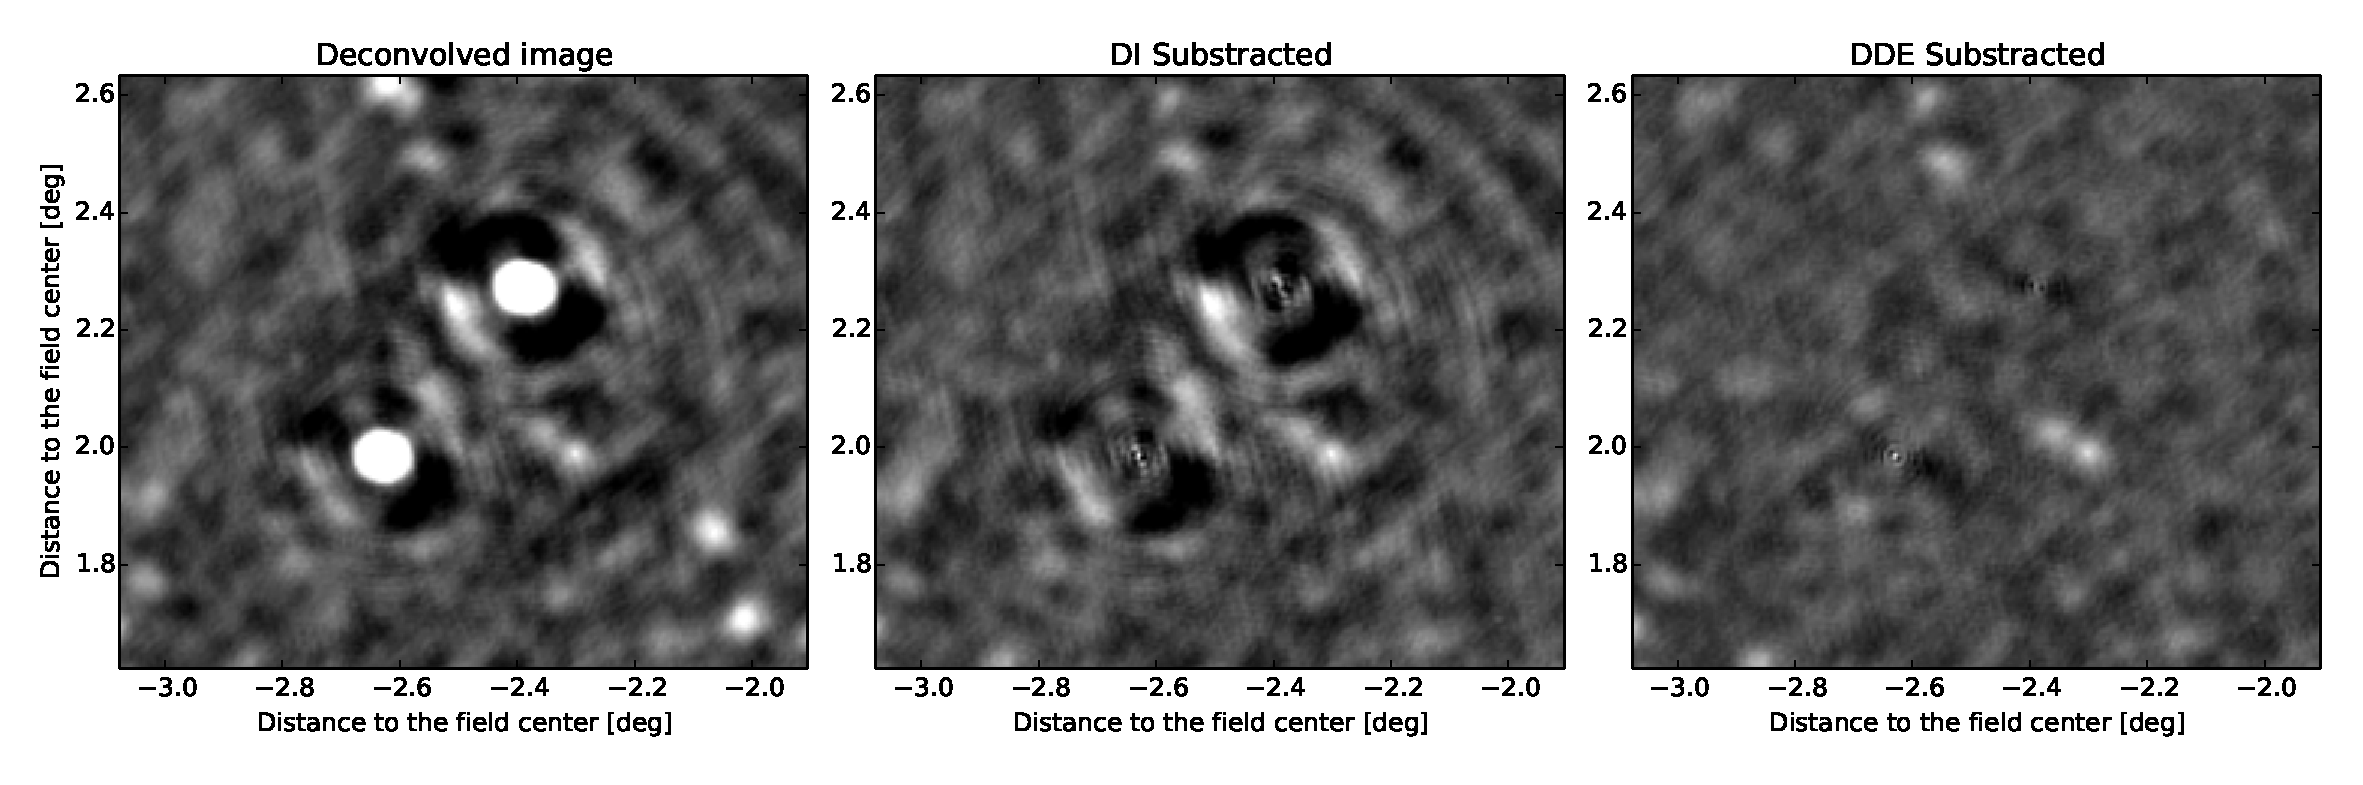
\includegraphics[width=\textwidth]{residZoom}
\caption{\label{fig:resid} This figure shows compares the image
  (left), the residuals data after simple skymodel substraction
  (center), and the residuals data after substracting the
  sky model corrupted by the direction-dependent solution (right).}
\end{center}
\end{figure*}


We test the ``DD-Stefval'' algorithm described above on a LOFAR observation of 3C295. The
visibilities produced by this interferometer are predominantly affected by direction dependent effects including (i) the phased beam instability and deviation from the
theoritical model, (ii) ionosphere time delays shifts, and (iii) Faraday rotation.

We first calibrate the dataset using BBS, and in order to build a pertinent model of the field, we substract 3C295. We extract the
sources using pyBDSM. The sources are the clustered in 10 directions using Voronoitesselation (fig. \ref{fig:tessel}). In Fig \ref{fig:resid}, we compare the residuals as
computed by substracting the model data in the visibility domain, and the model data affected by DDEs.




\begin{figure}[]
\begin{center}
%\hspace*{-1.3cm}
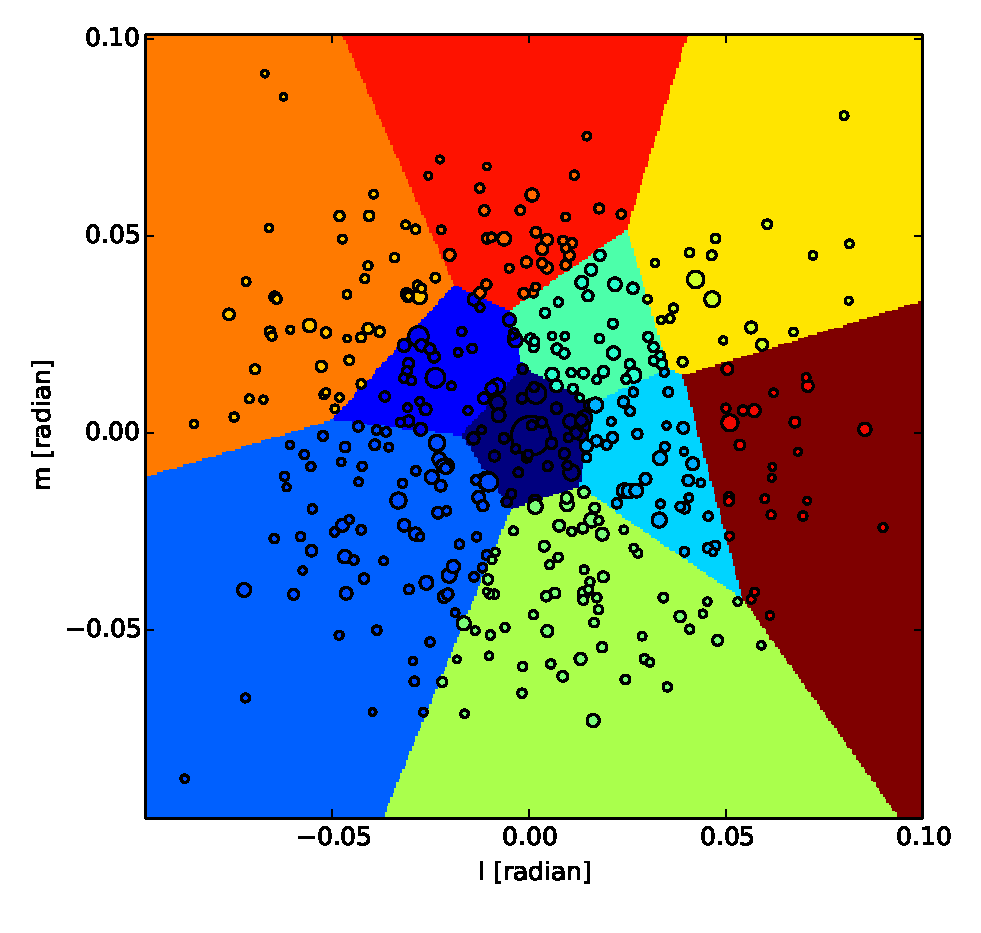
\includegraphics[width=\columnwidth]{tessel}
\caption{\label{fig:tessel} In order to minimize the number of degrees
of freedom, and increase the amount of signal in each direction, we cluster the sources in 10 direction using a Voronoi
tesselation.}
\end{center}
\end{figure}



\label{sec:realdata}

\section*{Conclusions}

Complexity $O(\mathrm{chicken}).$ Chicken!

Embarassingly parallel. GPU. Chicken!

Many variations possible, describes previous algorithms as special cases (approximations). Chicken!

Unifying framework? Chicken!

\bibliographystyle{mn2e}
\bibliography{cjpaper}

\appendix

\section{Deriving $4\times4$ operator representations}
\label{sec:4x4app}

This section contains the technical derivations needed for Sect.~\ref{sec:pol:DI}, and demonstartes how the
operator notation used therein maps onto the conventional matrix approach.

\subsection{Basic operators}

First, let us introduce the vectorization operator ``vec'' and its inverse in the usual way, e.g. for a $2\times2$ matrix:

\newcommand{\VEC}[1]{\mathrm{vec}\,{#1}}
\newcommand{\VECINV}[1]{\mathrm{vec}^{-1}\,{#1}}

\[
\VEC{\mat{X}} = \Matrix{c}{x_{11}\\x_{12}\\x_{21}\\x_{22}},~~~
\VECINV{\Matrix{c}{x_{11}\\x_{12}\\x_{21}\\x_{22}}} = \mat{X},
\]

This sets up a trivial isomorphism between the space of $2\times2$ complex matrices $\COMPLEX^{2\times2}$ and $\COMPLEX^4$. 
Any linear operator on $\mat{X} \in \COMPLEX^{2\times2}$ must be equivalent to multiplication of $\VEC{\mat{X}} \in \COMPLEX^4$ by 
a $4\times 4$ complex matrix. To put this formally, the $\mathrm{vec}$ operator induces an isomorphism 
$\mathrm{W}$ between $\COMPLEX^{4\times4}$ and the space of linear operators on $\COMPLEX^{2\times2}$:

\begin{eqnarray}
&& \mathrm{W}:\COMPLEX^{4\times4}\to\mathrm{Lin}(\COMPLEX^{2\times2},\COMPLEX^{2\times2}) \nonumber\\
&& \mathrm{W}(\mat{A})[\mat{X}] = \VEC{(\mat{A}\VEC{\mat{X}})} \label{eq:iso:W}
\end{eqnarray}

Of particular interest to us are three linear operators on $\COMPLEX^{2\times2}$: right multiply by $\mat{A}$, left multiply by $\mat{A}$, and
transpose: 

\[
\begin{array}{l@{~}l}
\Rop{\mat{A}}[\mat{X}] &= \mat{XA} \\
\Lop{\mat{A}}[\mat{X}] &= \mat{AX} \\
\Top[\mat{X}] &= \mat{X}^T
\end{array}
\]

Being linear, these operators must have a $4\times4$ matrix representation in $\COMPLEX^4$. 
Indeed, if $\mat{Y}=\Rop{\mat{A}}[\mat{X}]$, then 

\begin{equation}
\Matrix{c}{y_{11}\\y_{12}\\y_{21}\\y_{22}} = \VEC{\Rop{\mat{A}}[\mat{X}]} = 
\Matrix{cccc}{a_{11}&a_{21}&0&0 \\ a_{12}&a_{22}&0&0 \\ 0&0&a_{11}&a_{21} \\ 0&0&a_{12}&a_{22} }
\Matrix{c}{x_{11}\\x_{12}\\x_{21}\\x_{22}} 
\end{equation}

Likewise, 

\begin{equation}
\VEC{\Lop{\mat{A}}[\mat{X}]} = 
\Matrix{cccc}{a_{11}&0&a_{12}&0 \\ 0&a_{11}&0&a_{12} \\ a_{21}&0&a_{22}&0  \\ 0&a_{21}&0&a_{22} }
\VEC{\mat{X}},
\end{equation}

and

\begin{equation}
\VEC{\Top[\mat{X}]} = 
\Matrix{cccc}{1&0&0&0 \\ 0&0&1&0 \\ 0&1&0&0 \\ 0&0&0&1} \VEC{\mat{X}}.
\end{equation}

Since $(\mat{A}\mat{X})^T = \mat{X}^T \mat{A}^T$, the superposition of a transpose and
an $\Lop{\mat{A}}$ or $\Rop{\mat{A}}$ operator is equivalent to the opposite-hand operator using $\mat{A}^T$:

\begin{eqnarray}
\label{eq:LA:RATT}
\big[ \Rop{\mat{A}^T}[\cdot] \big ]^T = \Lop{\mat{A}}[\cdot] ~~&~&~~
\big[ \Lop{\mat{A}}[\cdot] \big]^T = \Rop{\mat{A}^T}[\cdot] \nonumber\\
\big[ \Rop{\mat{A}^H}[\cdot] \big ]^T = \Lop{\bar{\mat{A}}}[\cdot] ~~&~&~~
\big[ \Lop{\bar{\mat{A}}}[\cdot] \big]^T = \Rop{\mat{A}^H}[\cdot],
\end{eqnarray}

which we can also write as e.g.

\begin{equation}
\label{eq:RATT:op}
\Lop{\mat{A}} = \Top \Rop{\mat{A}^T},~~~\Top\Lop{\mat{A}} = \Lop{\mat{A}^T}.
\end{equation}

We may repurpose the symbols $\Top$, $\Rop{\mat{A}}$ and $\Lop{\mat{A}}$ to represent the $4\times4$ matrices above. It
is easy to see that Eq.~\ref{eq:RATT:op} must necessarily hold for the $4\times4$ matrix forms as well.

Note that the meaning of $\Top$ is specifically a transpose in $\COMPLEX^{2\times2}$ space -- it is not the same
thing as a transpose of the $4\times4$ matrices. What $\Top$ actual does in $\COMPLEX^4$ is a swapping of vector 
elements (i.e. swapping of rows 2 and 3). 

Other obvious properties are:

\begin{equation}
\label{eq:RAB:LAB}
\Lop{\mat{A}}\Lop{\mat{B}} = \Lop{\mat{AB}},~~~\Rop{\mat{A}}\Rop{\mat{B}} = \Rop{\mat{BA}},~~~[\Rop{\mat{A}}]^{-1} = \Rop{\mat{A^{-1}}}
\end{equation}

The above equations are true whether interpreted as operators, or as $4\times4$ matrix products.

\subsection{Derivatives and Jacobians}

A matrix-valued function of a matrix $\mat{F}(\mat{G})$, $\mat{F}:\COMPLEX^{2\times2}\to\COMPLEX^{2\times2}$ has a natural
representation as a vector-valued function of a vector, $\bmath{f}:\COMPLEX^4\to\COMPLEX^4$:

\[
\bmath{f}(\bmath{g}) = \VEC{\mat{F}(\VECINV{\bmath{g}})}.
\]

The partial and conjugate partial Jacobians of $\bmath{f}$ with respect to $\bmath{g}$ ($\bar{\bmath{g}}$) are then $4\times4$ matrices (Eq.~\ref{eq:Jk}):

\[
\JJ_g = [ \partial f_i / \partial g_j ],~~~\JJ_{\bar{g}} = [ \partial f_i / \partial \bar{g}_j ]
\]

We can now use the isomorphism of Eq.~\ref{eq:iso:W} to formally define the corresponding ``''Wirtinger derivative operators'' 
of $\mat{F}$ with respect to $\mat{G}$ and $\mat{G^H}$ as

\begin{equation}
\label{eq:def:dF:dG}
\frac{\partial\mat{F}}{\partial{\mat{G}}} = \mathrm{W}(\JJ_g),~~~
\frac{\partial\mat{F}}{\partial{\mat{G}^H}} = \Top \mathrm{W}(\JJ_{\bar{g}})
\end{equation}

This definition allows to formulate the Jacobians of Sect.~\ref{sec:pol:DI} (see e.g. Eq.~\ref{eq:JJtop}) 
in terms of matrices of operators. In particular, it is easy to see (just from considering the corresponding $4\times4$ matrices) that 

\[
\frac{\partial(\mat{GA})}{\partial{\mat{G}}} = \Rop{A},~~~~\frac{\partial(\mat{AG^H})}{\partial{\mat{G^H}}} = \Lop{A}.
\]

\subsection{Row reordering and the transpose}

Equation~\ref{eq:JJ} builds the full complex Jacobian from the partial Jacobian components. It is important to note that
once constructed, the rows of such a Jacobian matrix may be arbitrarily reshuffled, as long as we reshuffle the components of the residuals 
vector in exactly the same way, and vice versa.

A particularly useful reshuffle corresponds to the $\Top$ operator above (i.e. to a transpose in $\COMPLEX^{2\times2}$ space). We exploit this
in Eq.~\ref{eq:RRtranspose} to re-write the reshuffle the residuals vector (in $\COMPLEX^{4\Nbl}$ space) so that its bottom half represents
to the matrices given by $\mat{R}^H$ (rather than simply the element-by-element conjugate $\bar{\mat{R}}$). Propagating this reshuffle into
the Jacobian is equivalent to applying $\Top$ to every operator in the bottom half of the Jacobian. Conveniently, as shown by Eq.~\ref{eq:LA:RATT} above, this turns
the $\mathcal{R}$ operator into  $\mathcal{L}$, and vice versa.

\subsection{Conjugating the Jacobian}

The complex Jacobian given in operator notation of Eq.~\ref{eq:JJ:pol} is a matrix of $2\Nbl\times2\Na$ operators. Its equivalent in conventional
notation is a matrix of $8\Nbl\times8\Na$ complex numbers, in which each $4\times4$ block of complex numbers corresponds to one operator 
(via the $\mathrm{W}$ isomorphism defined above).






\label{lastpage}

\end{document}